\begin{frame}{2024 DQ Checks}
    \begin{itemize}
        \item Look at all of 2024 Data and compare it to 2023
        \item Focus was on the Track Variables
        \item Expected good agreements?
        \item But agreements weren't straightforward
        \begin{itemize}
            \item Variables like Positions were fine.
            \item Momenta were not
            \item Most variables were quite different
            \item Attributed to the changed background and changed optics
            \item Made one to one correspondence with 2023 data difficult
        \end{itemize}
    \end{itemize}
\end{frame}

\begin{frame}{2024 DQ Checks -- Some Plots}
    \begin{itemize}
        \item We knew the beam crossing angle changed 
        \item From -160 $\mu$rad in 2023 to +160 $\mu$rad in 2024 
    \end{itemize}
    \begin{columns}
        \begin{column}{0.5 \textwidth}
            \begin{figure}
                \centering
                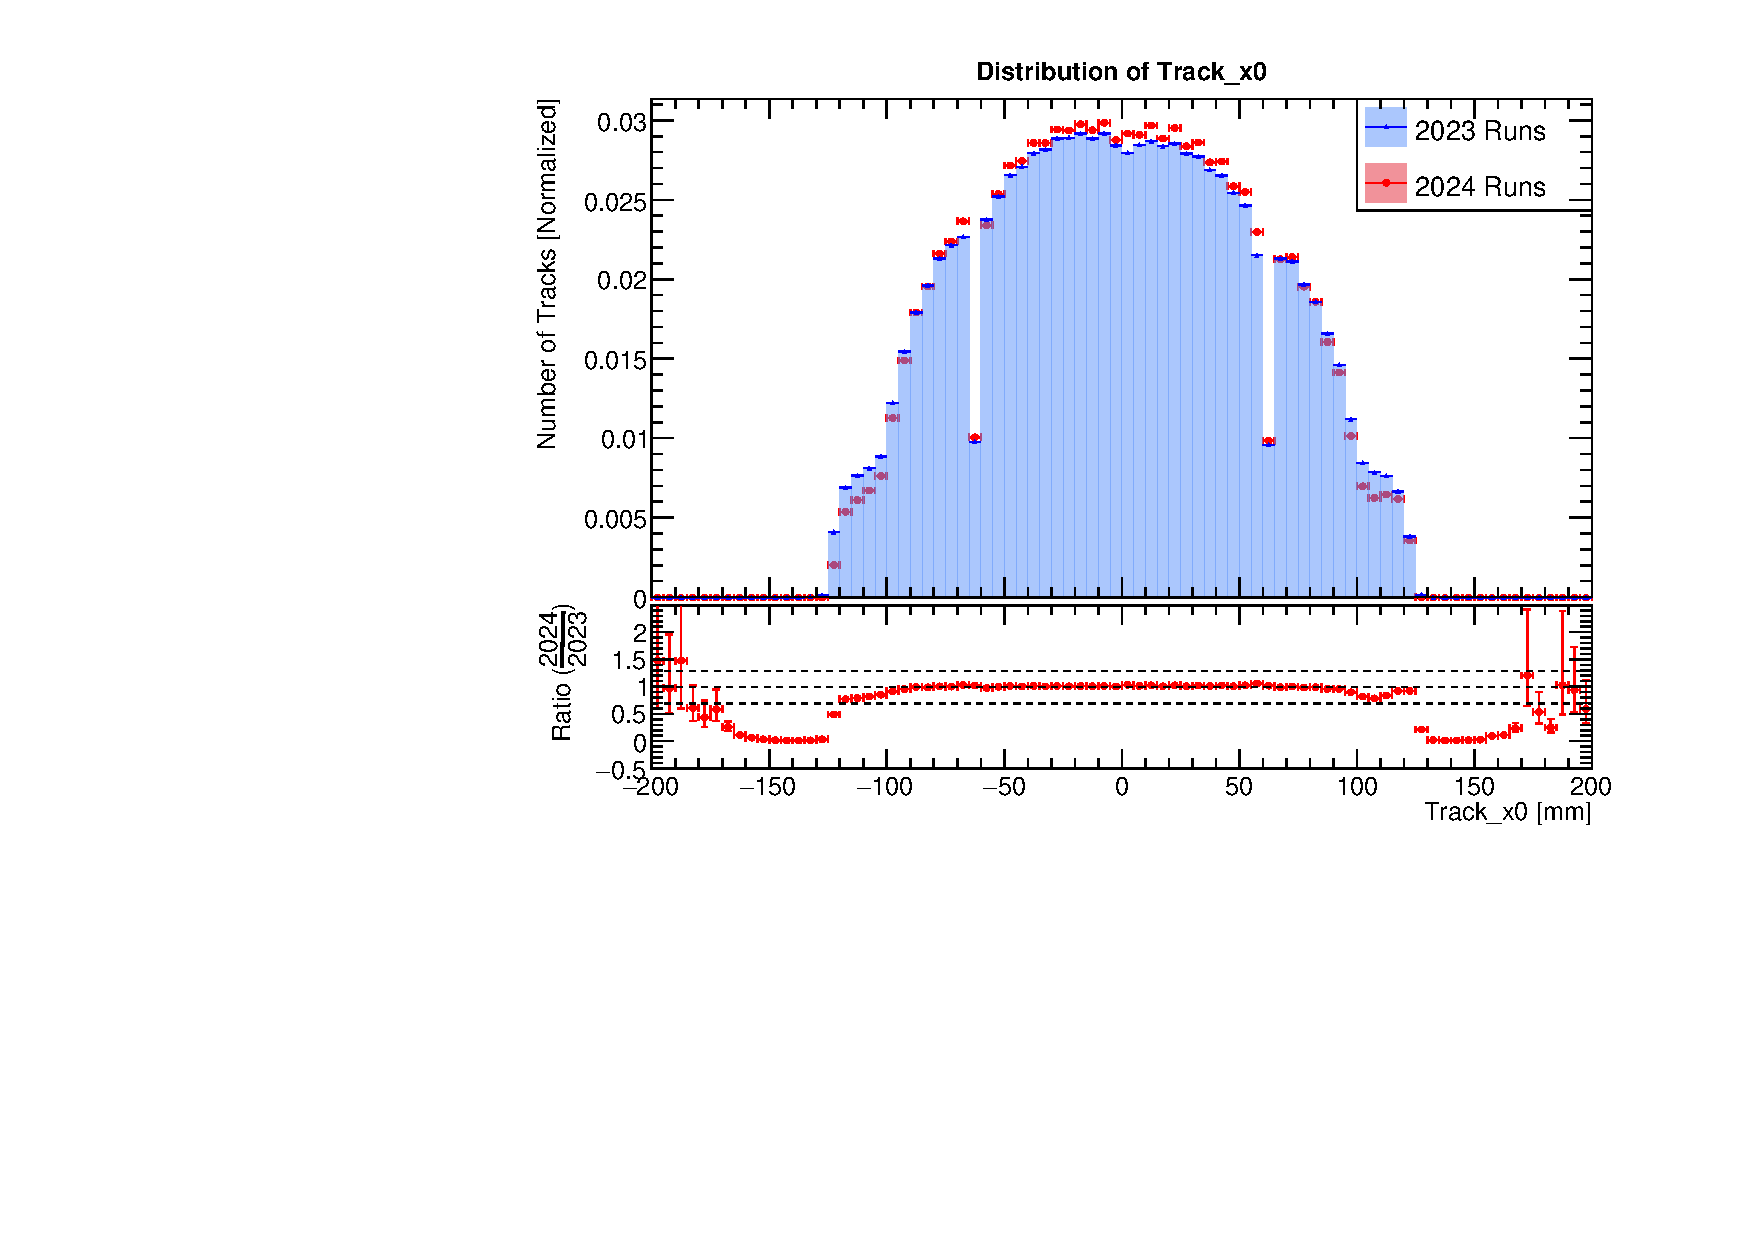
\includegraphics[width=\textwidth]{assets/Track_x0.pdf}
                \caption{Track x0}
            \end{figure}
        \end{column}
        \begin{column}{0.5 \textwidth}
            \begin{figure}
                \centering
                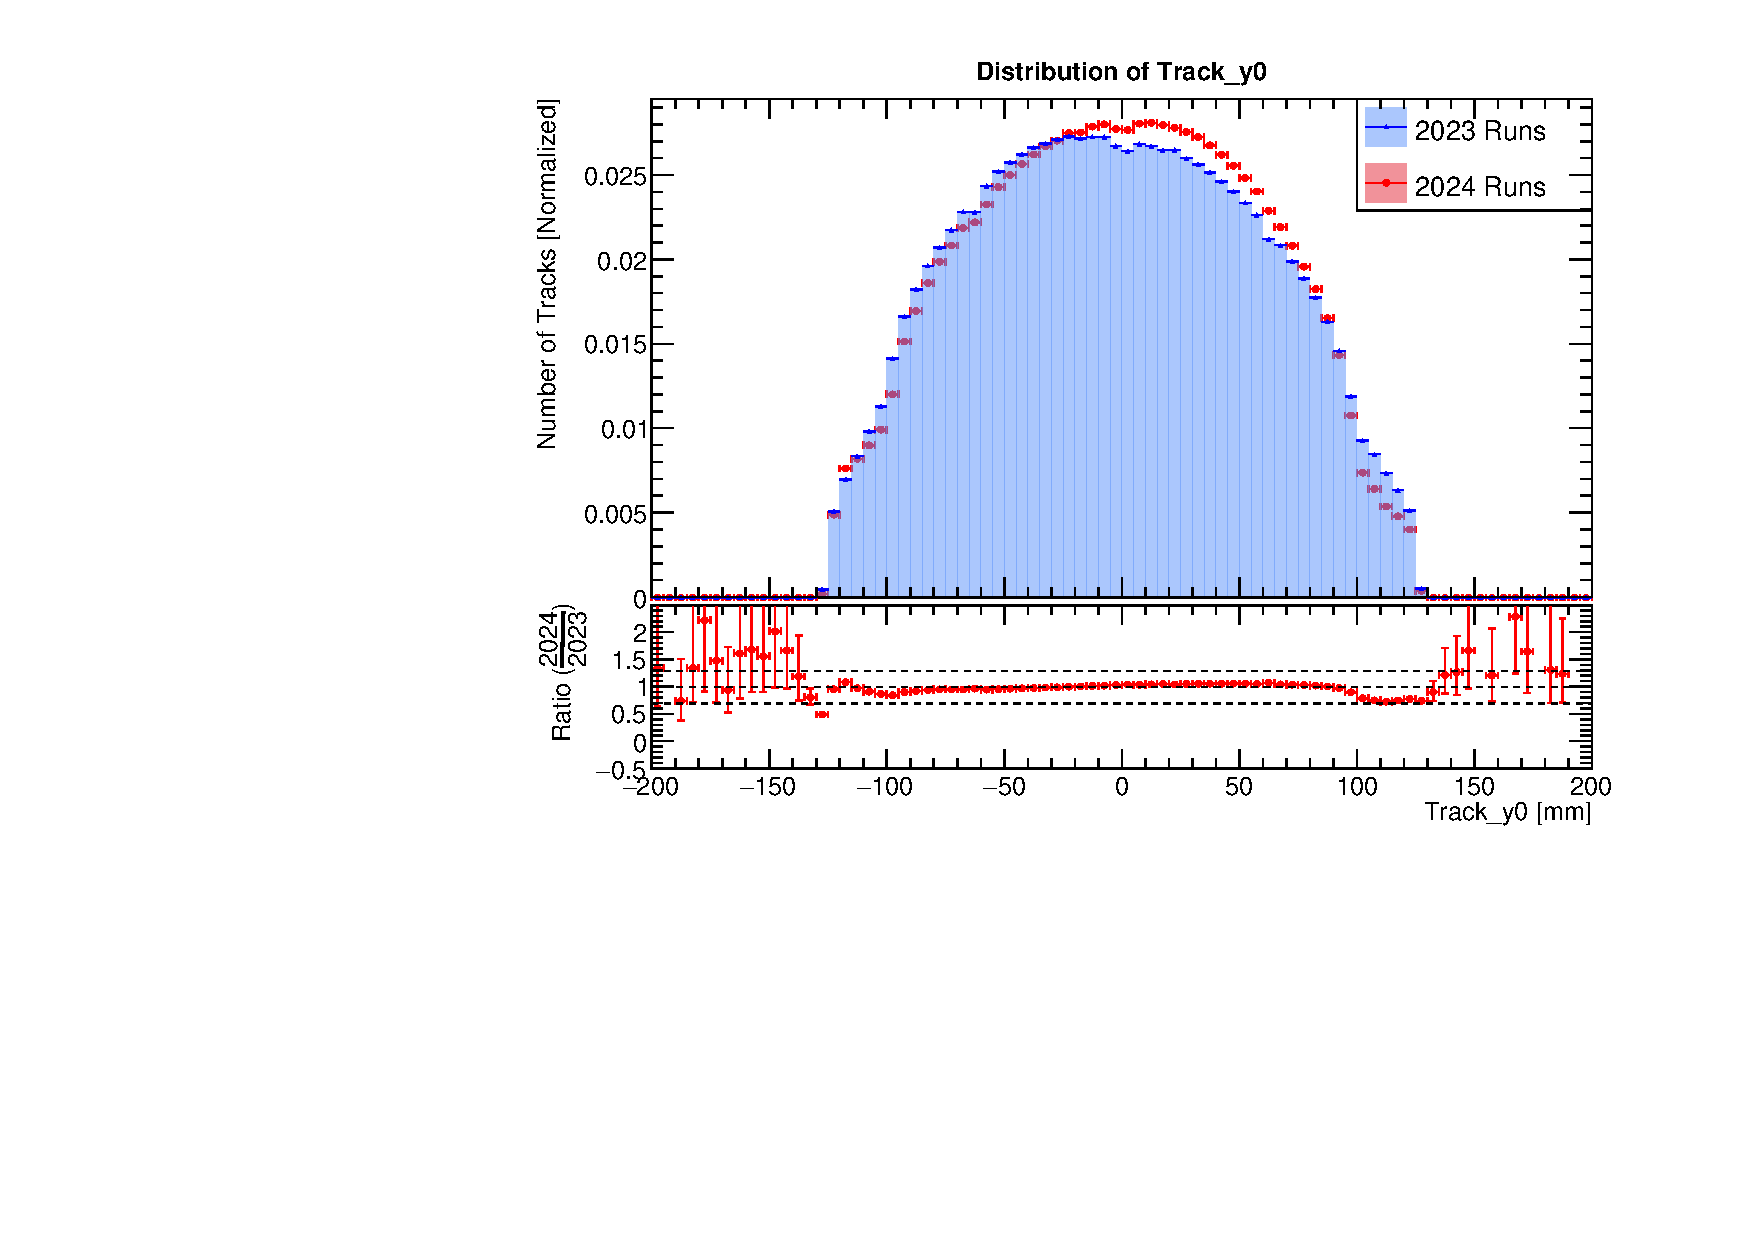
\includegraphics[width=\textwidth]{assets/Track_y0.pdf}
                \caption{Track y0}
            \end{figure}
        \end{column}
    \end{columns}
    \begin{itemize}
        \item We observed the corresponding shift in the the track positions
    \end{itemize}
\end{frame}

\begin{frame}{2024 DQ Checks -- Some Plots}
    \begin{itemize}
        \item That had huge implications on the observed background
    \end{itemize}

        \begin{figure}
            \centering
            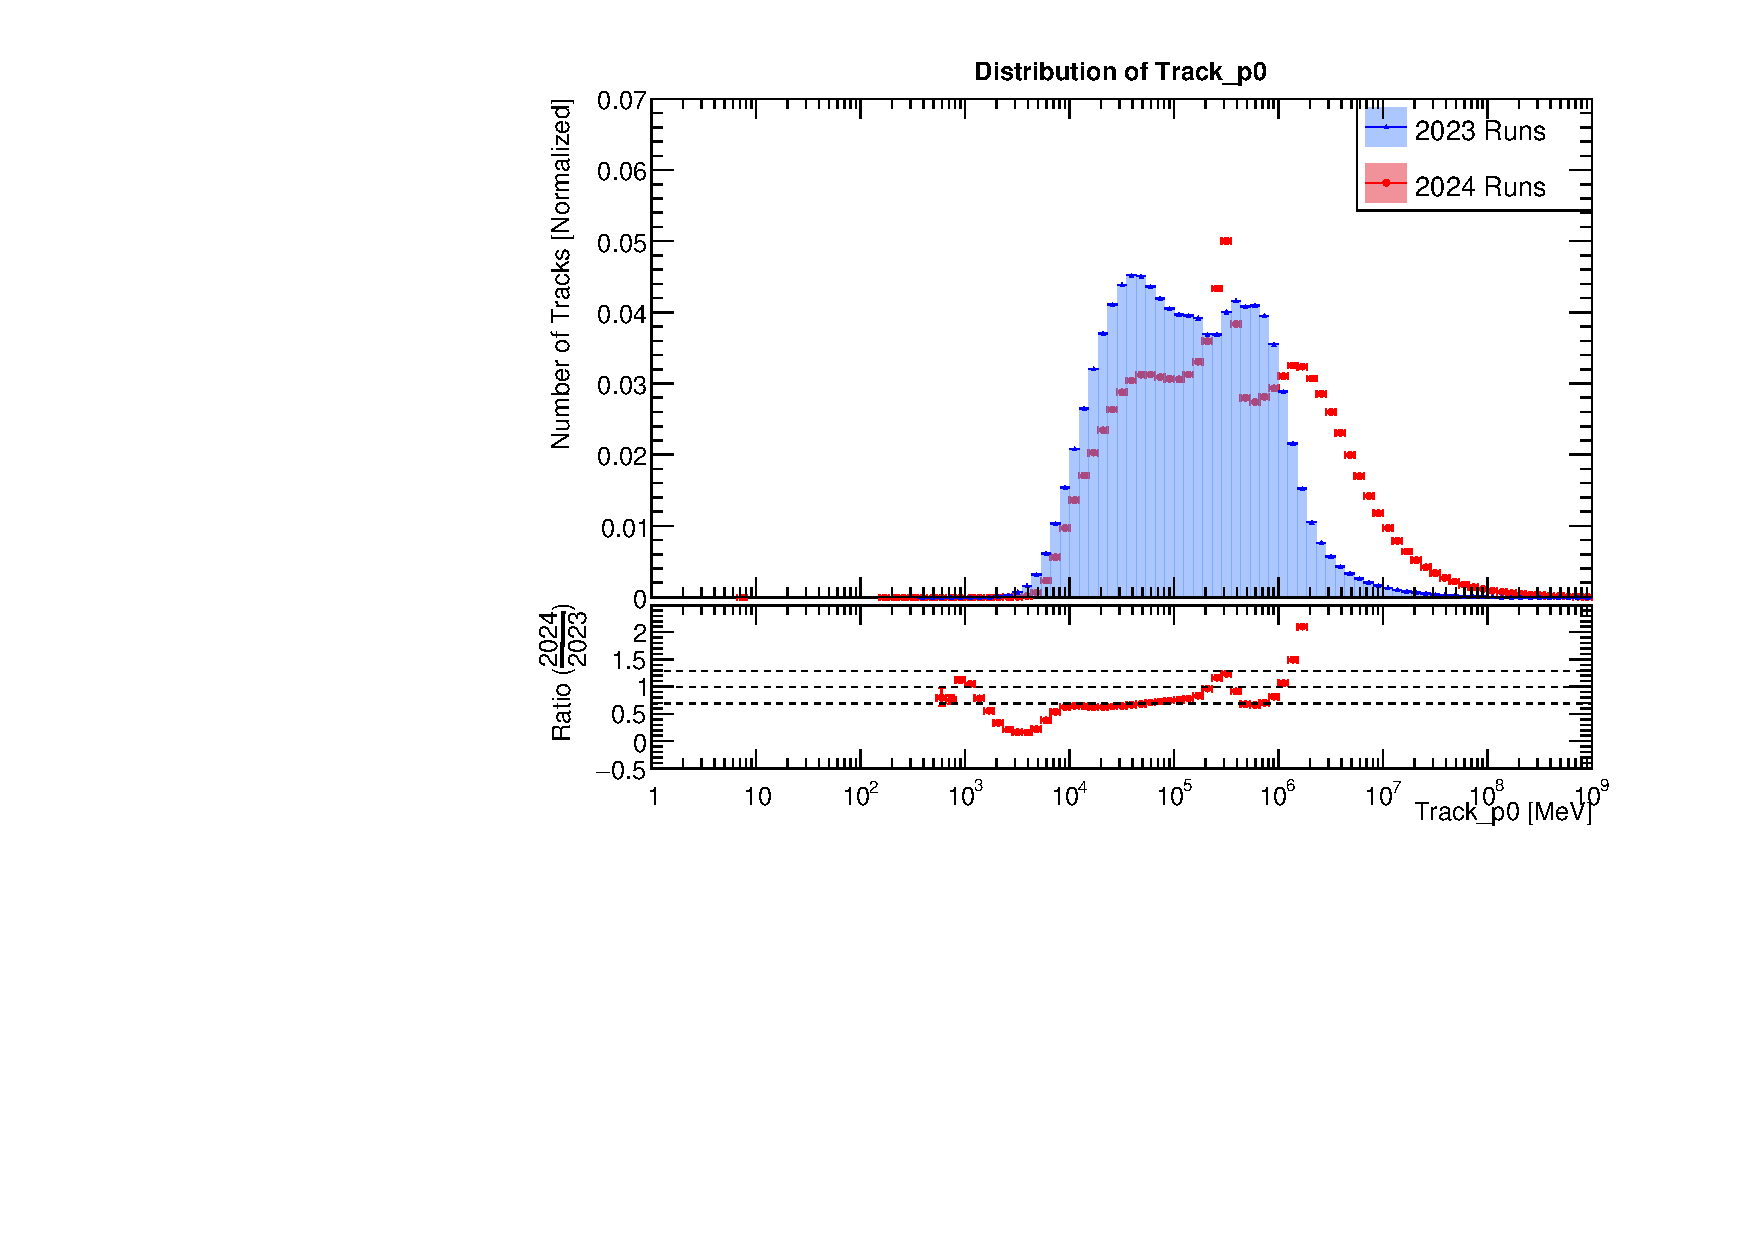
\includegraphics[width=0.7\textwidth]{assets/Track_p0.pdf}
            \caption{Track p0}
        \end{figure}
    \begin{itemize}
        \item A lot more high-momenta-positively charged muons in 2024
        \item This had non-trivial effects on the other track parameters
    \end{itemize}
\end{frame}

% \begin{frame}{Assimilate Comments from the Email}
%     \begin{itemize}
%         \item Do momenta binning for have a more equitable correspondence between 2023 and 2024
%         \item 
%     \end{itemize}
% \end{frame}

\begin{frame}{Follow Up on 2024 DQ Checks}
    \begin{itemize}
        \item Do a momentum binning to see if we can have a more equitable correspondence between 2023 and 2024
        \item Some new variables were introduced in the 2024 data
        \begin{itemize}
            \item module\_eta0, module\_phi0 
            \item which describes the first tracking module hit by the track
        \end{itemize}
    \item Start looking at the track parameters as a function of the starting module of the track
    \item Also needed updates to the 2024 run-list [Preliminary]
    \item Updates to the Yield Plots 
    \item Comparative analysis between four run periods in 2024
    \item Should be sent out early next week for feedback
    \end{itemize}
\end{frame}


\begin{frame}{2024 DQ Followup -- Some Plots}
\begin{columns}
    \begin{column}{0.7 \textwidth}
        \begin{figure}
            \centering
            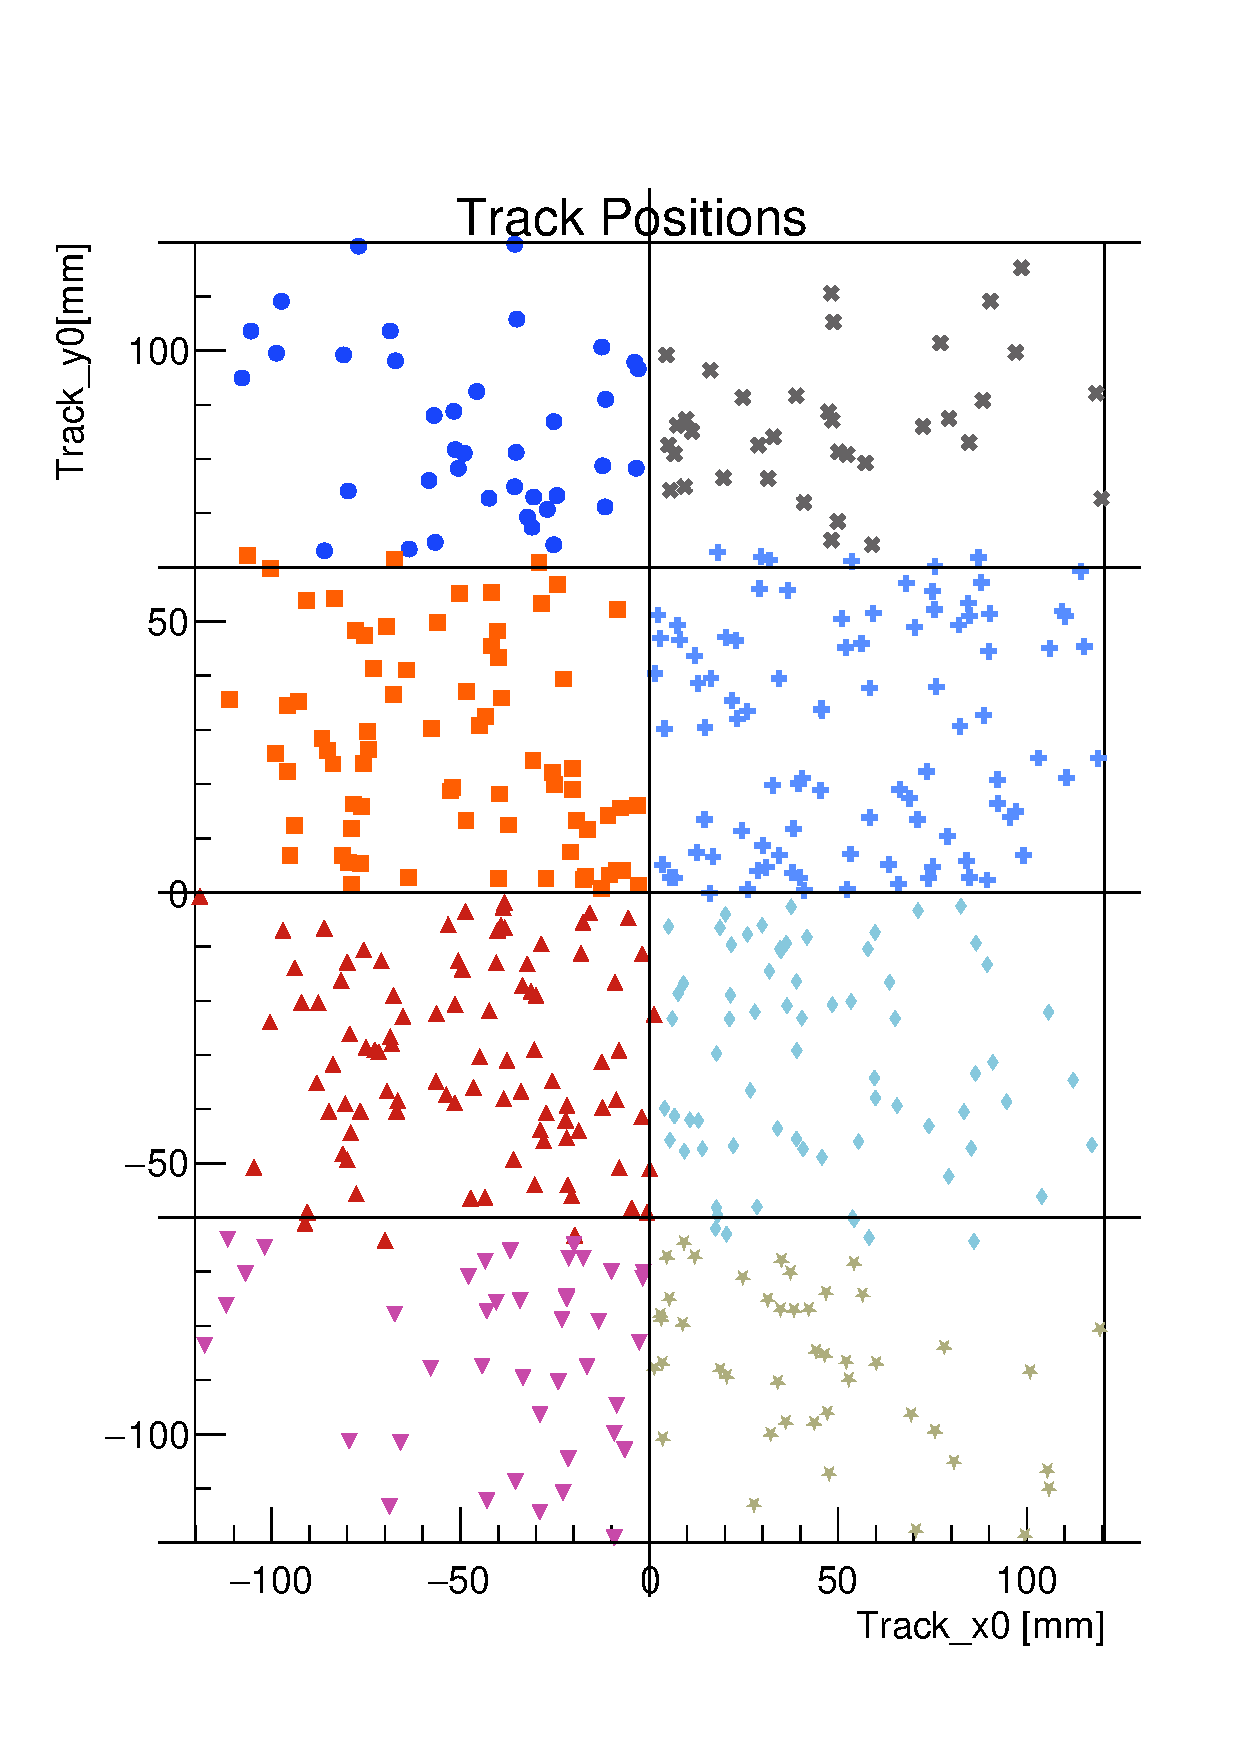
\includegraphics[height=0.7\textheight]{assets/Positions_st0_truemodule0.pdf}
            \caption{Track Points across Module}
        \end{figure}
    \end{column}
    \hspace{-2cm}\begin{column}{0.6 \textwidth}
        \begin{figure}
            \centering
            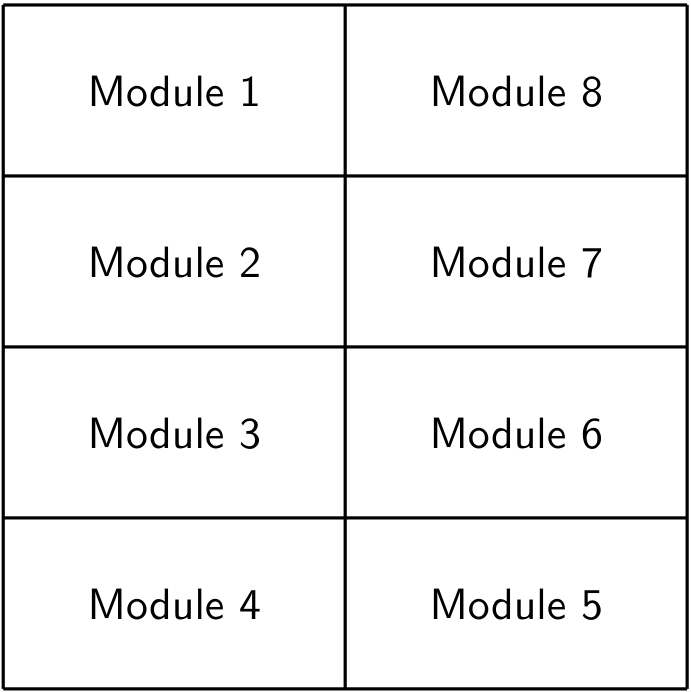
\includegraphics[height=0.4\textwidth]{assets/ModuleThumbnail.png}
            \caption{Module Numbering}
        \end{figure}
        \begin{itemize}
            \scriptsize
            \item Four central modules : 2,7,3,6
            \item Four outer modules : 1,8,4,7
        \end{itemize}
    \end{column}
\end{columns}
\end{frame}

\begin{frame}{2024 DQ Followup -- Some Plots}
    \begin{itemize}
        \small
        \item Wanted to see in which module the track ends up in the 3rd station
    \end{itemize}
    \begin{columns}
        \begin{column}{0.5\linewidth}
            \begin{figure}
                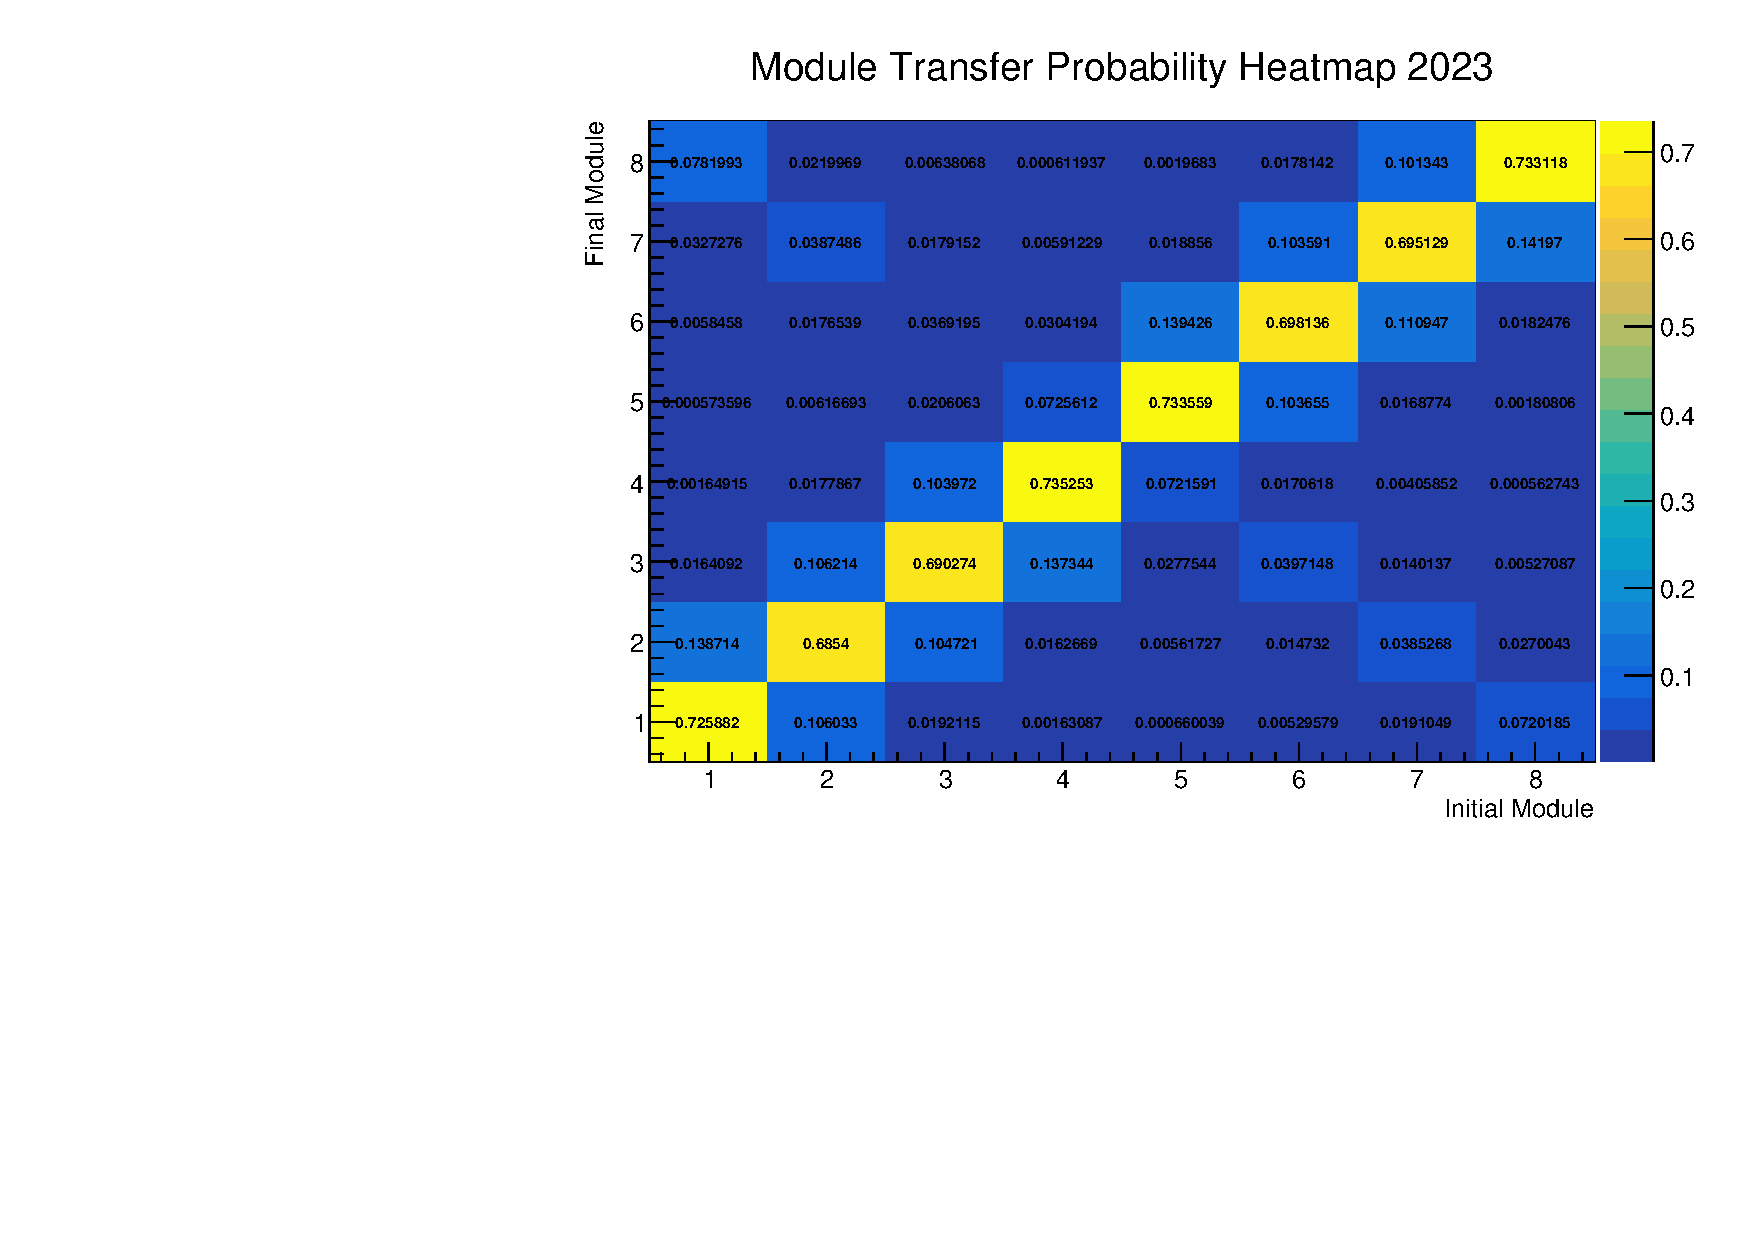
\includegraphics[width=\linewidth]{assets/st0_module_number vs st1_module_number_prob_2023.pdf}
                \caption{Probability of Transfer to a final module given a starting module [2023 data]}
            \end{figure}
        \end{column}
        \begin{column}{0.5\linewidth}
            \begin{figure}
                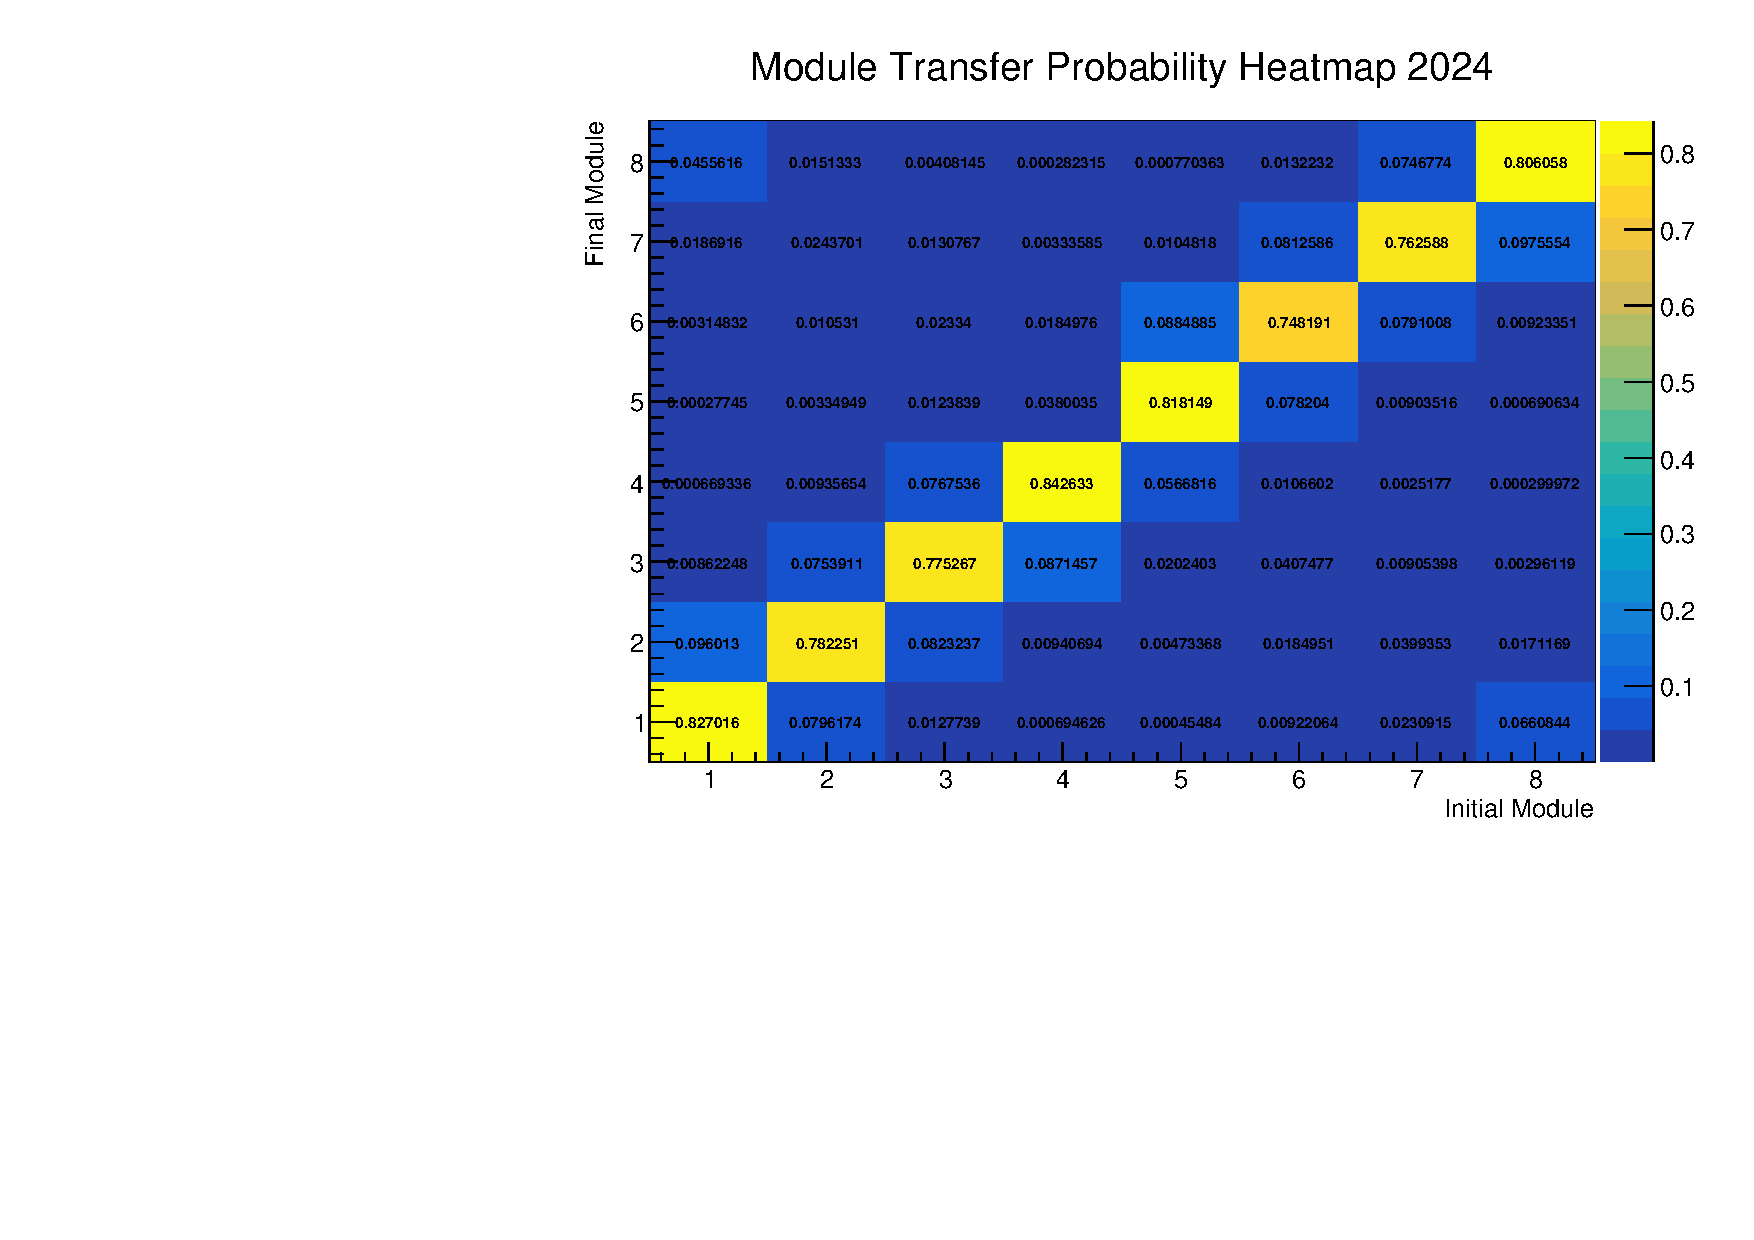
\includegraphics[width=\linewidth]{assets/st0_module_number vs st1_module_number_prob_2024.pdf}
                \caption{Probability of Transfer to a final module given a starting module [2024 data]}
            \end{figure}
        \end{column}
    \end{columns}
    \begin{itemize}
        \item We mostly transfer to the same final module 
        \begin{itemize}
            \item Some transfers to the module  top/below
            \item Some transfers to module on left/right (diagonal line)
        \end{itemize}
    \end{itemize}
\end{frame}


\begin{frame}{2024 DQ Followup -- Some Plots}
    \begin{figure}
        \centering
        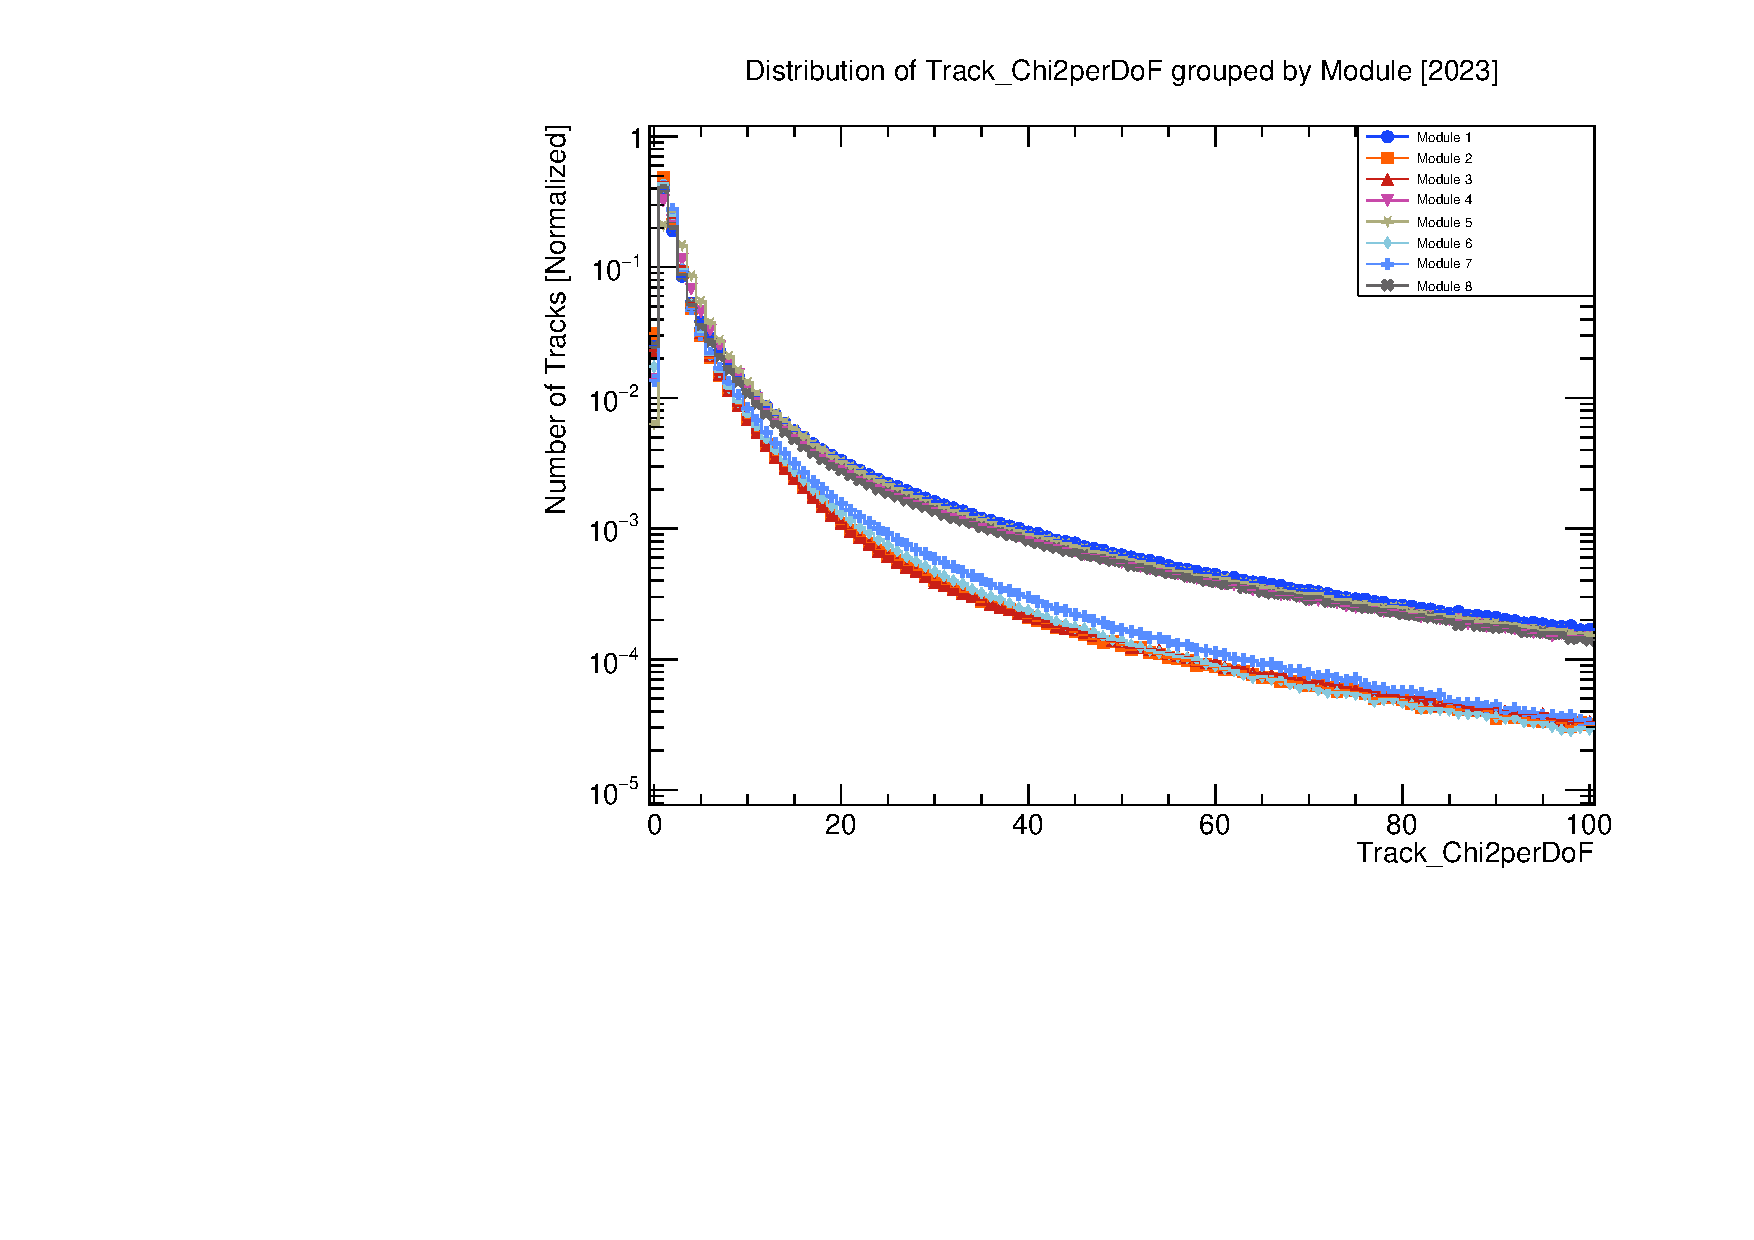
\includegraphics[width=0.7\textwidth]{assets/Track_Chi2perDoF_st0_2023.pdf}
        \caption{Track Points across Module}
    \end{figure}
    \begin{itemize}
        \item Some of the parameters factor out nicely with the central/outer module definition
    \end{itemize}
\end{frame}
